\documentclass{article}
\usepackage[utf8]{inputenc}
\usepackage{amsmath}
\usepackage{float}
\usepackage{listings}
\usepackage[pdftex]{graphicx}
\usepackage{amssymb}
%--------------------------------------------------------------------

\author{Pratik Aghor}
\title{Fourier and Chebyeshev Spectral Methods for 2D Swift-Hohenberg Equation}
\date{\today}  % Toggle commenting to test

\begin{document}

\maketitle
%--------------------------------------------------------------------
\section{Equation, Notation and Preliminaries:}
%-------------------------------------------------------------------
%-------------------------------------------------------------------
We consider 2d Swift-Hohenberg equation with quadratic-cubic nonlinearity (2dSH23), see \cite{swift1977hydrodynamic, cross1993pattern, lloyd2008localized}
\begin{equation}\label{eq:2dSH23}
 u_{t} =  -(1+\nabla^{2})^{2}u - \mu u + \nu u^{2} - u^{3}
\end{equation}

A dynamical-systems representation of the same Eqn.(\ref{eq:2dSH23}) is as follows:
\begin{align}\label{eq:2dSH23_abstract}
\begin{split}
 u_{t}  &=  Lu + N(u)\\
 L(u)   &= -(1+\nabla^{2})^{2}u - \mu u \\
 N(u)   &= \nu u^{2} - u^{3}
\end{split}
\end{align}

The domain $(x,y)\in[0, Lx] \times [0, Ly]$ is given. In Fourier spectral we will assume periodic boundary conditions (BC's) in both $x-$ and $y-$ directions. 


For computational purposes, we will need to transform the physical domain $x \in [0, 1]$ to a computational domain $x_{c} \in [xcmin, xcmax]$. This can be achived via a simple linear transformation given by
\begin{align}\label{eq:x2xc_abstract}
 \begin{split}
  x_{c} &= a_{1}x + b_{1}\textrm{, }y_{c} = a_{2}y + b_{2}\\
  b_{1}     &= xcmin\textrm{, }a_{1}     = (xcmax-xcmin)/L_{x}\\
  b_{2}     &= ycmin\textrm{, }a_{2}     = (ycmax-ycmin)/L_{y}
 \end{split}
\end{align}

Here, it will be given by:
\begin{align}\label{eq:x2xc}
 \begin{split}
  x_{c} &= a_{1}x + b_{1} \textrm{, } y_{c} = a_{2}y + b_{2}\\
  b_{1}     &= 0 \textrm{, } a_{1} = (2\pi)/L_{x}\\
  b_{2}     &= 0 \textrm{, } a_{2}     = (2\pi)/L_{y}
 \end{split}
\end{align}
And to get back from computational domain $x_{c}$ to the physical domain $x$, we need  the inverse of the above transformation:
\begin{equation}\label{eq:xc2x}
 x = (x_{c}-b_{1})/a_{1}
\end{equation}


Using chain rule, we can tranform the derivatives with respect to (henceforth wrt) $x$ into derivatives wrt $x_{c}$. 

\begin{align*}
 \begin{split}
  u_{x} &= u_{x_{c}} \frac{dx_{c}}{dx}\\
        &= a_{1} u_{x_{c}}\\
  u_{xx}&= \frac{\partial}{\partial x_{c}} \bigg\{u_{x_{c}} \frac{dx_{c}}{dx} \bigg\}\frac{dx_{c}}{dx}\\
        &= (a_{1})^{2} u_{x_{c} x_{c}}\\
  u_{yy}&= \frac{\partial}{\partial y_{c}} \bigg\{u_{y_{c}} \frac{dy_{c}}{dy} \bigg\}\frac{dy_{c}}{dy}\\
        &= (a_{2})^{2} u_{y_{c} y_{c}}        
 \end{split}
\end{align*}

Henceforth, we will use the modified version of the original Eqn(\ref{eq:2dSH23_abstract}) on the computational domain to develop the scheme:

\begin{align}\label{eq:2dSH23_computational}
\begin{split}
 u_{t}  &=  Lu + N(u)\\
 L(u)   &= -\bigg(1+a_{1}^{2}\frac{\partial^{2} }{\partial x^{2}} + a_{2}^{2}\frac{\partial^{2} }{\partial y^{2}} \bigg)^{2}u - \mu u\\
 N(u)   &= \nu u^{2} - u^{3}
\end{split}
\end{align}

For time integration, the second-order (two step) Adams-Moulton method for the linear term and the second-order (two-step) Adams-Bashforth method for the nonlinear term are used (Henceforth called AM2AB2).

The AM2AB2 algorithm reads:
\begin{subequations}\label{eq:AM2AB2}
 \begin{equation}
  \frac{u^{n+1}-u^{n}}{\Delta t} = L \frac{u^{n+1} + u^{n}}{2} + \frac{3}{2} N(u^{n}) - \frac{1}{2} N(u^{n-1})
 \end{equation} 
 \begin{equation}
  \bigg( I - \frac{\Delta t}{2} L \bigg) u^{n+1} = \bigg( I + \frac{\Delta t}{2} L \bigg)u^{n} + \frac{3 \Delta t}{2} N(u^{n}) - \frac{\Delta t}{2} N(u^{n-1})
 \end{equation}
\end{subequations}



%-------------------------------------------------------------------
%-------------------------------------------------------------------
\section{Fourier Spectral}
%-------------------------------------------------------------------
%-------------------------------------------------------------------
We begin with developing the formalism from Eqn.(\ref{eq:2dSH23_abstract}). First of all, we need to tranform the physical domain into $x_{c} \in [0, 2\pi]$, where the $c$ stands for `computational'.

From Eqn.(\ref{eq:x2xc}), we get
\begin{align}\label{eq:x2xc_Fourier}
 \begin{split}
  x_{c} &= ax + b\\
  b     &= 0\\
  a     &= 2\pi
 \end{split}
\end{align}

We will try to discretize Eqn.(\ref{eq:2dSH23_computational}) on $x_{c}$. 

Transforming Eqn(\ref{eq:AM2AB2}) into Fourier space by taking a Fourier transform,  AM2AB2 algorithm reads:
\begin{equation}\label{eq:AM2AB2_Fourier}
 \bigg( I - \frac{\Delta t}{2} L \bigg) \hat{u}^{n+1} = \bigg( I + \frac{\Delta t}{2} L \bigg)\hat{u}^{n} + \frac{3 \Delta t}{2} N^{n} - \frac{\Delta t}{2} N^{n-1}
\end{equation}
Where $\hat{u} = fft_{x}(fft_{y}(u))$ ,and $N^{n}$ and$N^{n-1}$ are the coefficients in $fft_{x}(fft_{y}(N(u^{n})))$ and $fft_{x}(fft_{y}(N(u^{n})))$ respectively.
%-------------------------------------------------------------------
\subsection{Getting fft to work in python}
%-------------------------------------------------------------------
In order to see the oredring of Fourier modes in python, we do some trivial tests.

\begin{align*}
 \sin{x} &= \frac{e^{ix} - e^{-ix}}{2i}\\
 \cos{x} &= \frac{e^{ix} + e^{-ix}}{2}
\end{align*}

For $N$ grid points, assuming $N$ is even, the Fourier modes $\bar{k} \in [-N/2, N/2]$. In order to find the ordering of $\bar{k}$, we expect to see $ k_{1} = -0.5i$ and $k_{-1} = 0.5 i$ in the expansion of $\sin{x}$. In the expansion of $\cos{x}$, we expect to see $ k_{1} = 0.5$ and $k_{-1} = -0.5$, with all others being zero. 

Some results for different N's are as follows:
\begin{verbatim}
 u = sin(xc) 

N =  8 

v = fft(u) = 
[ 1.43029718e-18+0.00000000e+00j -7.08192362e-17-5.00000000e-01j
  1.53080850e-17-1.38777878e-17j  1.24474906e-17+0.00000000e+00j
  2.91858728e-17+0.00000000e+00j  4.02030662e-17+0.00000000e+00j
  1.53080850e-17+1.38777878e-17j -4.30636606e-17+5.00000000e-01j]
_____________________________________________________________________

u = cos(xc) 

N =  8 

v = fft(u) = 
[-4.30636606e-17+0.00000000e+00j  5.00000000e-01-8.61273212e-17j
  1.53080850e-17+0.00000000e+00j  0.00000000e+00+2.86059436e-18j
  1.24474906e-17+0.00000000e+00j  0.00000000e+00+2.48949813e-17j
  1.53080850e-17+0.00000000e+00j  5.00000000e-01+5.83717456e-17j]
_____________________________________________________________________

u = 2.0*sin(xc) + sin(3.0*xc) 

N =  4 

v = fft(u) = 
[ 1.5308085e-16+0.j  -1.5308085e-16-0.5j  1.5308085e-16+0.j
 -1.5308085e-16+0.5j]

_____________________________________________________________________

u = 2.0*sin(xc) + sin(3.0*xc) 

N =  8 

v = fft(u) = 
[-8.99930287e-17+0.00000000e+00j -1.32051576e-16-1.00000000e+00j
  7.65404249e-17+5.55111512e-17j -1.32051576e-16-5.00000000e-01j
  2.43073879e-16+0.00000000e+00j -2.10292737e-17+5.00000000e-01j
  7.65404249e-17-5.55111512e-17j -2.10292737e-17+1.00000000e+00j]
_____________________________________________________________________
\end{verbatim}

These tests clearly indicate that the $\bar{k}$ is arranged in the following manner:

$\bar{k} = [0, 1, 2, ..., (N/2)-1, N/2, (-N/2)+1, ..., -1]$, i.e., for $N = 8$, 
$\bar{k} = [0, 1, 2, 3, 4, -3, -2, -1]$. There is an obvious asymmetry apparent from this analysis. There is no $k = -4$ mode! If the solution would have been, say, a standing wave, we would never be able to capture it because we will never have enough modes to counter-balance the $k= N/2$ mode. Hence, we decide to forcefully put it to $0$.

From the analysis done in class, we know that the convergence of Fourier spectral method is faster than any algebraic power of $1/N$ (exponential convergence), especially with periodic BC's.

Hence, if we keep enough modes, we can zero-out the highest mode as the coefficients in the expansion of $u$ will drop off fast enough. This way, we keep the $\bar{k}$ symmetric in terms of positive and negative modes present and take $\bar{k} = [0, 1, 2, ..., (N/2)-1, 0, (-N/2)+1, ..., -1]$.

A detail needs to be mentioned here. In the above results, the grid $x_{c}$ did not include the last point. That is,

\begin{verbatim}
 xc = 
[0.         0.78539816 1.57079633 2.35619449 3.14159265 3.92699082
 4.71238898 5.49778714]
 
 N =  8
\end{verbatim}

\begin{verbatim} numpy fft \end{verbatim} function assumes periodic BC's and hence the last grid point need not be mentioned. In order to plot the results, we can pad the current xc with the value at the last grid-point. 

In order to test the 2d fft in python, consider 
\begin{align*}
 \sin {x} \cos{y} &= \big[\frac{e^{ix} - e^{-ix}}{2i}\big]\big[ \frac{e^{iy} + e^{-iy}}{2}\big]\\
                  &= -0.25 i \big[e^{ix}e^{iy} + e^{ix}e^{-iy} - e^{-ix}e^{iy} - e^{ix}e^{-iy}\big]
\end{align*}

Taking the outer product of $\sin {x}$ and $\cos{y}$ to get $u(x, y)$, the result I obtained was the following:
\begin{verbatim}
_____________________________________________________________________

Running python test_fft2.py... 

Nx x Ny =  4  x  4 

xc = 
[0.         1.57079633 3.14159265 4.71238898]
yc = 
[0.         1.57079633 3.14159265 4.71238898]
u(x, y) = sin(xc)cos(yc) 

u(x, y) = sin(xc)cos(2yc) 

v = fft2(u)/(Nx*Ny) = 
[[0.+0.j   0.+0.j   0.+0.j   0.+0.j  ]
 [0.+0.j   0.-0.25j 0.+0.j   0.+0.25j]
 [0.+0.j   0.+0.j   0.+0.j   0.+0.j  ]
 [0.+0.j   0.-0.25j 0.+0.j   0.+0.25j]]

 done!

_____________________________________________________________________
_____________________________________________________________________

Running python test_fft2.py... 

Nx x Ny =  8  x  8 

xc = 
[0.         0.78539816 1.57079633 2.35619449 3.14159265 3.92699082
 4.71238898 5.49778714]
yc = 
[0.         0.78539816 1.57079633 2.35619449 3.14159265 3.92699082
 4.71238898 5.49778714]
u(x, y) = sin(xc)cos(yc) 

u(x, y) = sin(xc)cos(2yc) 

v = fft2(u)/(Nx*Ny) = 
[[0.+0.j   0.+0.j   0.+0.j   0.+0.j   0.+0.j   0.+0.j   0.+0.j   0.+0.j  ]
 [0.+0.j   0.-0.25j 0.+0.j   0.+0.j   0.+0.j   0.+0.j   0.+0.j   0.+0.25j]
 [0.+0.j   0.+0.j   0.+0.j   0.+0.j   0.+0.j   0.+0.j   0.+0.j   0.+0.j  ]
 [0.+0.j   0.+0.j   0.+0.j   0.+0.j   0.+0.j   0.+0.j   0.+0.j   0.+0.j  ]
 [0.+0.j   0.+0.j   0.+0.j   0.+0.j   0.+0.j   0.+0.j   0.+0.j   0.+0.j  ]
 [0.+0.j   0.+0.j   0.+0.j   0.+0.j   0.+0.j   0.+0.j   0.+0.j   0.+0.j  ]
 [0.+0.j   0.+0.j   0.+0.j   0.+0.j   0.+0.j   0.+0.j   0.+0.j   0.+0.j  ]
 [0.+0.j   0.-0.25j 0.+0.j   0.+0.j   0.+0.j   0.+0.j   0.+0.j   0.+0.25j]]

 done!

_____________________________________________________________________


\end{verbatim}

Writing $u(x, y) = \sin{x_{c}}\cos{2y_{c}}$, the result I obtained was the following:

\begin{align*}
 \sin {x} \cos{2y} &= \big[\frac{e^{ix} - e^{-ix}}{2i}\big]\big[ \frac{e^{2iy} + e^{-2iy}}{2}\big]\\
                  &= -0.25 i \big[e^{ix}e^{2iy} + e^{ix}e^{-2iy} - e^{-ix}e^{2iy} - e^{ix}e^{-2iy}\big]
\end{align*}
\begin{verbatim}
 
Running python test_fft2.py... 

Nx x Ny =  8  x  8 

xc = 
[0.         0.78539816 1.57079633 2.35619449 3.14159265 3.92699082
 4.71238898 5.49778714]
yc = 
[0.         0.78539816 1.57079633 2.35619449 3.14159265 3.92699082
 4.71238898 5.49778714]
u(x, y) = sin(xc)cos(2yc) 

v = fft2(u)/(Nx*Ny) = 
[[0.+0.j   0.+0.j   0.+0.j   0.+0.j   0.+0.j   0.+0.j   0.+0.j   0.+0.j  ]
 [0.+0.j   0.+0.j   0.+0.j   0.+0.j   0.+0.j   0.+0.j   0.+0.j   0.+0.j  ]
 [0.+0.j   0.-0.25j 0.+0.j   0.+0.j   0.+0.j   0.+0.j   0.+0.j   0.+0.25j]
 [0.+0.j   0.+0.j   0.+0.j   0.+0.j   0.+0.j   0.+0.j   0.+0.j   0.+0.j  ]
 [0.+0.j   0.+0.j   0.+0.j   0.+0.j   0.+0.j   0.+0.j   0.+0.j   0.+0.j  ]
 [0.+0.j   0.+0.j   0.+0.j   0.+0.j   0.+0.j   0.+0.j   0.+0.j   0.+0.j  ]
 [0.+0.j   0.-0.25j 0.+0.j   0.+0.j   0.+0.j   0.+0.j   0.+0.j   0.+0.25j]
 [0.+0.j   0.+0.j   0.+0.j   0.+0.j   0.+0.j   0.+0.j   0.+0.j   0.+0.j  ]]

 done!

_____________________________________________________________________
\end{verbatim}

%-------------------------------------------------------------------
\subsection{Conclusions of fft tests:}
%-------------------------------------------------------------------

Note that in the above calculations, in the matrix $u$, the $i^{th}$ row corresponded to a fixed value of $y$, while each $j^{th}$ column corresponded to a fixed value of $x$. $u[i, j]\equiv u(y, x)$. We do this slightly counter-intuitive maneuver for computational simplification and so that the matrix $u$ aligns (somewhat) with the pictorial representation with $x$ axis going horizontal while $y$ being the vertical axis. Even after this, the direction in which $y$ increases and the direction in which the index $i$ increases are opposite to each other. While plotting solutions, we should take note of this.    

Above numerical experiments suggest that if $v = \textrm{fft2}(u)/N_{x}N_{y}$, then $v[i, j]$ corresponds to $(k_{y}[i], k_{x}[j])$ modes.

%-------------------------------------------------------------------
\subsection{Testing 2d Heat Equation:}
%-------------------------------------------------------------------
Tested the code for the $2d$ heat equation. 
\begin{equation}\label{eq:2dheat}
 u_{t} =  \nabla^{2}u 
\end{equation}

\begin{figure}[H]
        \centering
        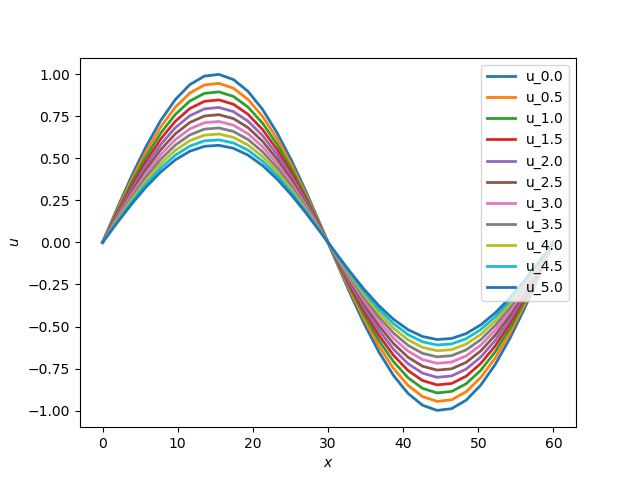
\includegraphics[scale = 0.6]{Figs/ut_heat_fourier.png}
            \caption{$2d$ heat equation test}
        \label{fig:2d_heat_test}
\end{figure}

%-------------------------------------------------------------------
\subsection{Results}
%-------------------------------------------------------------------
%-------------------------------------------------------------------
The parameters were chosen to be $\mu = 0.5$ and $\nu = 2.2$, while the domain was chosen to be $L_{x} \times L_{y} = 9\pi \times 9\pi$. 
The discretization was $ N_{y} \times N_{x} = 64 \times 64$, with the timestep chosen to be $dt = 0.02$. The initial condition was $u(x, y) = 1 + \sin{x}\sin{y}$ which settled into the following state: 
\begin{figure}[H]
        \centering
        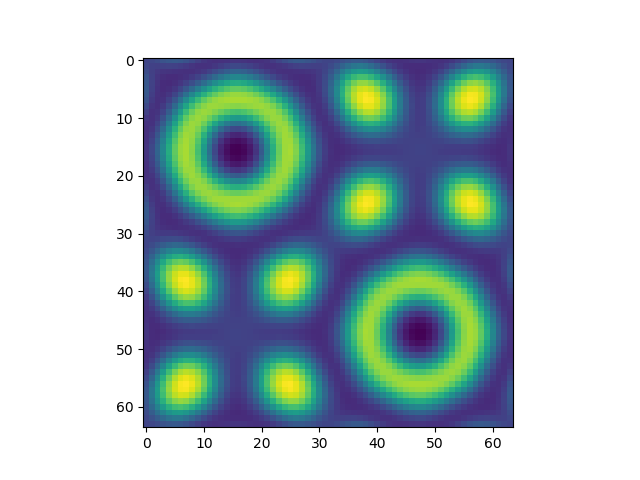
\includegraphics[scale = 0.6]{Figs/u40000.png}
            \caption{$2d$ Swift-Hohenberg}
        \label{fig:2d_heat_test}
\end{figure}

%-------------------------------------------------------------------

%-------------------------------------------------------------------
%--------------------------------------------------------------------
\bibliographystyle{apalike}
%\bibliographystyle{unsrt} % Use for unsorted references  
%\bibliographystyle{plainnat} % use this to have URLs listed in References
%\cleardoublepage
%\bibliography{References/references} % Path to your References.bib file

\bibliography{bib/references} % Path to your References.bib file
 \if@openright\cleardoublepage\else\clearpage\fi
 \cleardoublepage
 \pagestyle{empty}
%--------------------------------------------------------------------
\end{document}
